\documentclass[../report.tex]{subfiles}

\begin{document}
\subsection{Giới thiệu về HOG}
Histogram of Oriented Gradients (HOG) là một loại đặc trưng được dùng 
trong lĩnh vực thị giác máy tính và xử lý hình ảnh 
với mục đích phát hiện đối tượng \cite{tim-hieu-hog}. 
Các khái niệm về HOG được nêu 
ra từ năm 1986 tuy nhiên cho đến năm 2005 HOG mới được sử dụng 
rộng rãi sau khi Navneet Dalal và Bill Triggs công bố những 
bổ sung về HOG. Hog tương tự như các biểu đồ edge 
orientation, scale-invariant feature transform descriptors 
(như sift, surf,..), shape contexts nhưnghog được tính toán 
trên một lưới dày đặc các cell và chuẩn hóa sự tương phản 
giữa các block để nâng cao độ chính xác. \\
Ý tưởng chính trong đặc trưng HOG là hình dạng và trạng thái 
của vật thể được đặc trưng bằng sự phân bố của gradient 
và hướng của cạnh. \\
Đặc trưng HOG được tính trên một vùng, do sự 
biến thiên về màu sắc của các vùng là khác nhau, kết quả là mỗi vùng sẽ cho ta một vector đặc trưng của nó.

\subsection{Các bước thực hiện tính HOG}
Thuật toán tính toán đặc trưng HOG gồm 5 bước chính:
\begin{itemize}
\item B1: Chuẩn hóa hình ảnh trước khi xử lý.
\item B2: Tính độ lớn và góc gradient của các thành phần ảnh.
\item B3: Phân chia ảnh thành các cell và block. 
Lấy phiếu bầu để sinh ra vector đặc trưng cho từng cell.
\item B4: Tính toán vector đặc trưng cho mỗi block.
\item B5: Tổng hợp vector đặc trưng của block để tạo ra 
vector cuối cùng là đặc trứng HOG của ảnh 
\end{itemize}

\subsubsection{Chuẩn hóa hình ảnh}
Đầu tiên cắt lấy phần ảnh muốn chọn sao cho các ảnh có 
kích thước cố định (VD: $64 \times 128$ pixels) \\[3mm]
Tiếp theo là chuẩn hóa giá trị các pixel. 
Bước chuẩn hóa này hoàn toàn 
không bắt buộc, nhưng trong một số trường hợp, 
bước này có thể cải thiện hiệu suất của bộ mô tả HOG. 
Có ba phương pháp chuẩn hóa chính mà chúng ta có thể xem xét:
\begin{itemize}
\item Chuẩn hóa Gamma/lũy thừa: lấy $\log(p)$ của mỗi 
pixel $p$ trong ảnh đầu vào.
\item Chuẩn hóa căn bậc hai: lấy $\sqrt{p}$
của mỗi pixel $p$ trong ảnh đầu vào.
\item Chuẩn hóa phương sai (Variance normalization): Đưa các giá trị 
pixel trong ảnh về dạng phân bố chuẩn $(0,1)$.
\end{itemize}

\subsubsection{Tính độ lớn và góc gradient của các thành phần ảnh}
Có thể sử dụng bộ lọc $D_x = [-1 \quad 0 \quad 1]$, 
$D_y = [-1 \quad 0 \quad 1]^T$. Hoặc phổ biến hơn là bộ lọc Sobel. 
\\[3mm]
Xác định góc của vector gradient, có thể xác định 
theo kiểu “có dấu” hoặc “không dấu”. 
\\[3mm]
Với ảnh màu:
\begin{itemize}
\item Tính gradient theo chiều $x$, $y$ 
cho mỗi kênh màu (RGB có 3 kênh màu). 
\item Với mỗi kênh màu, chọn gradient lớn nhất, 
lấy độ lớn của vector đó và góc là góc của vector lớn nhất đó.  
\item Mỗi pixel khi đó chỉ còn biểu diễn bởi 2 giá trị.
\end{itemize}

\subsubsection{Phân chia ảnh thành các cell và block. 
Lấy phiếu bầu để sinh ra vector đặc trưng cho từng cell}
Mỗi hình ảnh được phân chia thành nhiều khối, 
các khối này có thể đặt chồng lên nhau, 
khoảng cách giữa hai khối liên tiếp là bằng nhau. \\[3mm]
Mỗi khối gồm nhiều ô. Mỗi ô có kích thước bằng nhau, 
số lượng ô trong các khối là bằng nhau. \\[3mm]
Ví dụ: \\
Nếu ta có một hình ảnh 128 x 128 với  \\
pixel\_per\_cell = 4 x 4 thì sẽ có 32 x 32 = 1024 cell,  \\
pixel\_per\_cell = 32 x 32, sẽ có 4 x 4 = 16 cell. 
\begin{figure}[H]
\centering
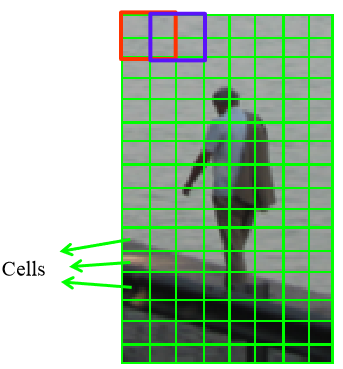
\includegraphics[width=10cm]{figures/cell-block.png}
\end{figure}
\noindent Với mỗi ô (cell), ta chia không gian góc thành 
các bin (thường là 9 ứng với mỗi bin là góc 20 độ).
\\[3mm]
Mỗi pixel trong ô (cell) được vote vào biểu đồ, 
trọng số của mỗi vote chính là cường độ gradient tại pixel đó.
\begin{figure}[H]
\centering
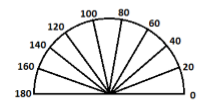
\includegraphics[width=7cm]{figures/bins-degree.png}
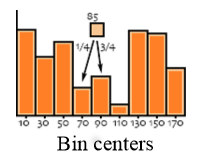
\includegraphics[width=7cm]{figures/bins.png}
\end{figure}

\subsubsection{Tính toán vector đặc trưng cho mỗi block}
Ghép vector đặc trưng của từng cell lại với nhau và 
chuẩn hóa sẽ cho ta vector đặc trưng của block. 
\\[3mm]
Chuẩn hóa có thể theo chuẩn L1 hoặc L2. 
\\[3mm]
Ví dụ một block có kích thước 16x16 pixel: \\
\tab Cell kích thước $8 \times 8$ pixel, 9 bin gradient. \\
\tab Mỗi block gồm 4 cell.  \\
\tab Vector đặc trưng của mỗi block gồm $9 \times 4 = 36$ thành phần.

\subsubsection{Tính toán vector đặc trưng của toàn bộ ảnh}
Ghép vector đặc trưng của từng block lại với nhau 
và chuẩn hóa sẽ cho ta vector đặc trưng của ảnh. 
\\[3mm]
VD: Ảnh $64 \times 128$, cell $8 \times 8$, 
block $16 \times 16$, stride $8 \times 8$ thì vector đặc trưng của toàn ảnh có 
$7 \times 15 \times 36=3780$ chiều. 
\begin{figure}[H]
\centering
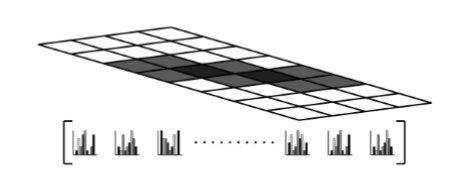
\includegraphics[width=13cm]{figures/feature-vector.png}
\end{figure}

\end{document}
